\documentclass[nonacm]{acmart}

%%
%% \BibTeX command to typeset BibTeX logo in the docs
\AtBeginDocument{%
  \providecommand\BibTeX{{%
    \normalfont B\kern-0.5em{\scshape i\kern-0.25em b}\kern-0.8em\TeX}}}

%%
%% These commands are for a JOURNAL article.
%% PLEASE IGNORE THEM!
\acmJournal{TOIT}
\acmVolume{37}
\acmNumber{4}
\acmArticle{111}
\acmMonth{8}

%%
%% end of the preamble, start of the body of the document source.
\usepackage{textcomp}
\usepackage{multirow}
\usepackage{array}
\usepackage{hyperref}
\usepackage{tabularx}
\usepackage{booktabs}


\newcolumntype{M}[1]{>{\centering\arraybackslash}m{#1}}
\newcommand{\bla}{blah blah blah blah blah blah blah blah blah blah blah blah blah blah blah blah}
%Definition of Colors - Start
\definecolor{xred}{RGB}{255,0,0}
\definecolor{xblue}{RGB}{68,114,196}
\definecolor{xgreen}{RGB}{0,176,80}
\definecolor{xpurple}{RGB}{112,48,160}
\definecolor{xorange}{RGB}{237,125,49}
%Definition of Colors - End

\setcopyright{none}
\settopmatter{printacmref=false} % Removes citation information below abstract
\renewcommand\footnotetextcopyrightpermission[1]{} % removes footnote with conference information in first column
\pagestyle{plain}

% Anpassung der Header-Höhe
\setlength{\headheight}{21pt}
\addtolength{\topmargin}{-7.64952pt}

\begin{document}

\title{Aufgabenstellung 1 Taucher}

\begin{figure}
    \centering
    
\includegraphics[width=0.5\textwidth]{fig/Fig1.png}
    \label{fig:title-image}
\end{figure}


\author{Harald Beier (\lowercase{2410781028@hochschule-burgenland.at})}

\author{\\Susanne Peer (\lowercase{2410781002@hochschule-burgenland.at})}

\author{\\Patrick Prugger (\lowercase{2410781029@hochschule-burgenland.at})}



%Je nach dem in welcher Sprache ihr euer Paper schreiben wollt, benutzt bitte entweder den Deutschen-Titel oder den Englischen (einfach aus- bzw. einkommentieren mittels '%')

\begin{abstract}
%Deutsch
\textbf{KURZFASSUNG:}
Die Kurzfassung bzw. der Abstract ist ca. so wie ein Kino-Trailer der erste Kontakt mit eurem Paper. Wenn der Trailer nicht gut ist, dann schaue ich mir den Kino-Film erst gar nicht an. Das gleiche gilt auch hier im Abstract, wenn dieser nicht gut ist, wird das Paper gar nicht gelesen. Dabei hat eine gute Kurzfassung / ein guter Abstract 150-300 Wörter und wird in der PAST-Tense geschrieben (nach dem die Arbeit durchgeführt wurde). Darum schreibt man die Kurzfassung / den Abstract auch erst zum Schluss, wenn das Paper bereits fertig geschrieben ist. In jeder Kurzfassung / jedem Abstract sollte man folgende Struktur verfolgen:
\begin{itemize}
	\item\textbf{1-2 Sätze:} Beschreibt in welchem Universum / Forschungsfeld sich das Position Paper befindet
	\item\textbf{1-2 Sätze:} Beschreibt die Problemstellung in diesem Universum / Forschungsfeld
	\item\textbf{1-2 Sätze:} mit welcher Methodik / welchem Forschungsansatz schlägt ihr vor, um die Problemstellung zu bearbeiten?
	\item\textbf{1-2 Sätze:} Welches Ergebnis erwartet man sich bzw. welchen Mehrwert soll der Lösungsvorschlag bringen
	\item\textbf{1-2 Sätze:} Ausblick…was bedeutet das im “Big Picture”
\end{itemize}

%Englisch	
%\textbf{ABSTRACT:}
\end{abstract}

\maketitle

\newpage
%Je nach dem in welcher Sprache ihr euer Paper schreiben wollt, benutzt bitte entweder den Deutschen-Titel oder den Englischen (einfach aus- bzw. einkommentieren mittels '%')

%Deutsch
\section{Einleitung und Problemhintergrund}

Moderne Smart Offices nutzen heutzutage vermehrt Internet der Dinge / Internet of Things (IoT) und 
und Künstliche Intelligenz (KI) / Artificial Intelligence (AI), um Arbeitsumgebungen adaptiv zu	gestalten. 
Während bestehende Lösungen \cite{ref01} allgemeine Automatisierung bieten, fehlt es an zielgruppenspezifischer Anpassung
für neurodivergente Personen (z.B. Aufmerksamkeitsdefizit- / Hyperaktivitätsstörung (ADHS), Autismus) und Menschen 
die nach einem Burnout wieder an ihren Arbeitsplatz zurückkehren. Raumgestaltung muss multisensorisch gedacht werden, 
nicht nur Funktion und Ästetik prägen unsere Wahrnehmung, sondern auch Sinne wie z.B. Klang und Licht beeinflussen unsere 
Reaktion darauf.Die Arbeitswelt ignoriert bislang häufig, eine individuell angepasste Umgebung, um das Wohlbefinden zu 
stärken und produktives Potenzial zu entfalten. \\

Aktuelle Smart Office Lösungen sind auf Effizienz und Komfort ausgerichtet, 
berücksichtigen jedoch nicht, die heterogenen Bedürfnisse neurodivergenter Personen und 
Burnout-Rückkehrer:innen, zu adressieren. Studien zeigen, dass z.B. ADHS-Betroffene 
durch sensorische Überlastung (z.B. fluoreszierende Beleuchtung, plötzliche Geräusche) 
mehr zu Konzentrationsverluste neigen, als neurotypische Personen.
Trotz dieser Evidenz fehlen Lösungen, die Echtzeit-Anpassungen (z.B. dynamische Lichtsteuerung,
akustische Geräuschkulisse) ermöglichen.
Für Autist:innen sind unstrukturierte Arbeitsabläufe und spontane soziale Interaktionen,
eine zentrale Stressquelle. Bestehende Systeme bieten jedoch kaum Tools zur Visualisierung 
von Tagesplänen, oder zur Abschirmung von Unterbrechungen, obwohl dies die Produktivität 
steigern könnte. Gleichzeitig kämpfen Burnout-Rückkehrer:innen mit starren 
Arbeitszeitmodellen und unklaren Priorisierungen, die Rückfallrisiken erhöhen. Bei den
gewählten drei Userprofilen sind verschiedene Bedürfnisse und Herausforderungen zu
berücksichtigen, wo individuelle Anpassungen kontrolliert Reize steuern. \\

In diesem Paper wird ein Cloud-basierter Prototyp für ein Smart Office vorgestellt, dieser 
soll die identifizierten Lücken durch eine IoT-Architektur adressieren und eine Umgebungsanpassung 
in Echtzeit ermöglicht. 
Ein Dashboard soll je nach Userprofil Funktionalitäten, wie z.B. Aufgabenpriorisierung,
Tagesplänen, Raumstatus abbilden und Reizüberflutung präventiv entgegenwirken.
Durch individuelle Anpassungen (z.B. Licht, Musik, Raumtemperatur), welche in einem Userprofil
hinterlegt sind, können äußere Reize minimiert und die Produktivität, sowie das 
Wohlbefinden gesteigert werden. Weiters wird durch Sensoren eine dynamische Lichtsteuerung
ermöglicht, die sich u.a. an die jeweilige Tageszeit und äußere Lichteinstrahlung anpasst.\\
Die Architektur verzichtet auf komplexe Orchestrierung (Kubernetes) zugunsten 
schlanker Amazon Web Service (AWS)-Dienste. Nutzer:innen behalten via Opt-in-System die 
Kontrolle über ihre Daten, die ausschließlich lokal oder verschlüsselt im Simple Storage Service (S3) 
gespeichert werden sollen. Der Unterschied zu bestehenden Lösungen liegt in der 
Intersektionalität, statt isolierter Anpassungen integriert das System Parameter 
zur psychologischen Präventionsstrategien in eine einheitliche Plattform. \\

%%%%%%%%%%%%%%%%%%%%%%%%%%%%%%%%%%%%%%%%%%%%%%%%%%%%%%%%%%%%%%%%
%%% TODO: Feedback Igor -- Überlegt euch was und wie ihr evalierungen wollt:
%%%%%%%%%%%%%%%%%%%%%%%%%%%%%%%%%%%%%%%%%%%%%%%%%%%%%%%%%%%%%%%%
%Was -- Differenzierung -- Wie -- Vergleich mit bestehender Lösung , Referenzmatrix/-modell, DELTA Analyse 
%Performance -- Tools wie JMeter oder AWS CloudWatch würden sich glaub anbieten
%Ethik -- Was -- Einhaltung Privatsphäre -- Wie -- Ethik Review
%Usability -- Was -- Usability wie Verständlich ist das Dashboard aufgebaut -- Wie -- Befragung/Fragebogen -- eher ungeeignet für dieses Paper
%Barrierefreiheit -- Was -- WCAG konform?(https://www.w3.org/WAI/standards-guidelines/wcag/) -- Wie --automatisierte Accessibility Tests}
	
%%% https://wave.webaim.org/
%% https://www.deque.com/axe/

%%%%%%%%%%%%%%%%%%%%%%%%%%%%%%%%%%%%%%%%%%%%%%%%%%%%%%%%%%%%%%%%
%%{TODO Feedback Abschlussabsatz}
%%%%%%%%%%%%%%%%%%%%%%%%%%%%%%%%%%%%%%%%%%%%%%%%%%%%%%%%%%%%%%%%
%%Beim Position Paper wäre es schön, wenn ihr eure Einleitung mit folgendem Absatz beendet 
%%(das Beispiel ist auf Englisch....ihr müsst es natürlich auf Deutsch. machen):
%%The reminder of the position paper is organised as follows: Section 2 summarises the 
%%related work in the field. Next, in Section 3, we describe our experimental design where
%%we introduce an experimental testbed and explain how it could be used in a cost-benefit analysis.
%%Furthermore, we give an overview of potential stakeholders in an additive MaaS ecosystem including 
%%a profit sharing approach. Finally, in Section 4 we conclude our work and give an outline of 
%%future work in the field.
%%Ihr gebt also dem Leser einen Überblick, was als nächstes kommt, wenn er/sie weiterliest
	
%%%%%%%%%%%%%%%%%%%%%%%%%%%%%%%%%%%%%%%%%%%%%%%%%%%%%%%%%%%%%%%%
%%{TODO: Feedback Abschlussabsatz -- Erster Ansatz schnell zusammengeschrieben, bitte überarbeiten}
%%%%%%%%%%%%%%%%%%%%%%%%%%%%%%%%%%%%%%%%%%%%%%%%%%%%%%%%%%%%%%%%

In Abschnitt 2 wird zunächst ein Überblick über die bestehende Lösung und ein Einblick in den Bereich
der Smart Offices für neurodivergente Menschen und Burnout-Rückkehrer:innen gegeben. Abschnitt 3 stellt
das Konzept unseres Cloud-basierten Prototypen vor, der die identifizierten Lücken adressiert. Abschnitt 4 
schließt mit einer Diskussion möglicher Interessensgruppen und potenzielle Nutzer:innen und der Rolle
von präventiven psychologischen Strategien innerhalb des Systems. Abschließend wird in Abschnitt 5 wird 
dieses Projekt zusammengefasst und ein Ausblick auf zukünftige Forschungsmöglichkeiten gegeben, sowie mögliche 
Erweiterungen des Systems gegeben.

% Englisch
%\section{Introduction}

%%Ähnliche wie in der ersten Abgabe, gehört hier die Projekt-Idee mit zumindest folgenden Inhalten beschrieben:
%%\begin{itemize}
%%	\item\textbf{1. Absatz (Universum / Forschungsfeld): } \\
%%	Im ersten Absatz soll das Univsersum / Forschungsfeld beschrieben werden, in dem sich das Position Paper befindet. Der Leser / die Leserin soll aus dem "großen Ganzen" an die eigentliche Problemstellung herangeführt werden und wissen, in welchem Themenfeld sich diese befindet. \\
	
%%	\textbf{\textit{ACHTUNG}}: Es ist in Ordnung, wenn die Studierenden das Universum / Forschungsfeld in mehr als nur einem Absatz herleiten. Es ist nur wichtig, dass folgende Regel eingehalten wird: ein Absatz beteht zumindest aus 3 Sätzen, wobei ein Satz aus maximal 30 Worten besteht.\\
	
%%	\item\textbf{2. Absatz (Problemstellung im Universum / Forschungsfeld): } \\
%%	Im zweiten Teil wird dem Leser / der Leserin das Problem, welche im beschriebenen Universum / Forschungsfeld besteht, aufgezeigt bzw. beschrieben. Die Problemstellung gilt dabei als die Grundlage für das Position Paper, die hier beschrieben wird und die Methodik "WIE man es lösen würde" erklärt wird (in Kapitel 3). \\
	
%%	\textbf{\textit{ACHTUNG}}: Es ist in Ordnung, wenn die Studierenden die Problemstellung in mehr als nur einem Absatz herleiten. Es ist nur wichtig, dass folgende Regel eingehalten wird: ein Absatz beteht zumindest aus 3 Sätzen, wobei ein Satz aus maximal 30 Worten besteht.\\
	
%%	\item\textbf{3. Absatz (Lösungsansatz, um die Problemstellung zu bearbeiten): } \\
%%	Im 3. Teil soll eine Idee bzw. ein möglicher Lösungsansatz "angeteasert" werden, mit dem man die beschriebene Problemstellung bearbeiten möchte. Dabei ist es wichtig, dass der beschriebene Lösungsweg realistisch bzw. umsetzbar und auch nachvollziehbar ist. Es soll ein möglicher Weg sein, den man gehen kann, um die Problemstellung zu bearbieten oder sich zumindest einer Lösung anzunähern. Der Leser bzw. die Leserin soll den Eindruck bekommen, dass die Problemstellung tatsächlich damit lösbar sei. \\
	
%%	\textbf{\textit{ACHTUNG}}: Es ist in Ordnung, wenn die Studierenden den Lösungsansatz in mehr als nur einem Absatz herleiten. Es ist nur wichtig, dass folgende Regel eingehalten wird: ein Absatz beteht zumindest aus 3 Sätzen, wobei ein Satz aus maximal 30 Worten besteht.

%%	\item\textbf{Letzter Absatz (Aufbau des Position Papers): }\\
%%	Jedes Paper hat zum Schluss einen Absatz, der beschreibt, wie das vorliegende Position Paper aufgebaut ist. Hier ein Beispiel aus einem Position Paper, das auf Englisch geschrieben wurde: \\
	
%%	The remainder of this paper is organised as fol- lows: Section II summarises the related work in the field. Next, in Section III, we present the Security Evaluation Framework and explain how it can be used to evaluate the security of SDN-components. Furthermore, we show the general applicability of the proposed framework in an experimental study in Section IV. Finally, in Section V we conclude our work and give an outline of future work in the field.
	
%%\end{itemize}

%%\textbf{VORGABE}: dieses Kapitel soll genau eine A4-Seite benötigen

%%%%%%%%%%%%%%%%%%%%%%%%%%%%%%%%%%%%%%%%%%%%%%%%%%%%%%%%%%%%%%%%%%%%%%%%%%%%%%%%%%%%%%%%%%%%%%%
%%% THIS IS THE ORIGINAL ONE PAGER
%%%%%%%%%%%%%%%%%%%%%%%%%%%%%%%%%%%%%%%%%%%%%%%%%%%%%%%%%%%%%%%%%%%%%%%%%%%%%%%%%%%%%%%%%%%%%%%
%%\section{Einleitung und Problemhintergrund}

%%Bei der ersten Aufgabenstellung sollen die Studierenden ihre Projekt-Idee in Form
%%eines "One Pagers" (genau eine A4-Seite) beschreiben. Dabei sollen zumindest folgende
%%Informationen / Inhalte im "One Pager" beschrieben werden:


%%\begin{section}
	%%\textbf{Forschungsfeld: }
	%%Moderne Smart Offices nutzen heutzutage vermehrt Internet der Dinge / Internet of Things (IoT) und 
	%%und Künstliche Intelligenz (KI) / Artificial Intelligence (AI), um Arbeitsumgebungen adaptiv zu	gestalten. 
	%%Während bestehende Lösungen \cite{hasiwar2023towards} allgemeine Automatisierung bieten, fehlt es an zielgruppenspezifischer Anpassung
	%%für neurodivergente Personen (z.B. Aufmerksamkeitsdefizit- / Hyperaktivitätsstörung (ADHS), Autismus) und Menschen die nach einem Burnout wieder an ihren Arbeitsplatz zurückkehren. Raumgestaltung
	%%muss multisensorisch gedacht werden, nicht nur Funktion und Ästetik prägen unsere Wahrnehmung, sondern auch Sinne
	%%wie z.B. Klang und Licht beeinflussen unsere Reaktion darauf.	Die Arbeitswelt ignoriert bislang häufig, eine 
	%%individuell angepasste Umgebung, um das Wohlbefinden zu stärken und produktives Potenzial zu entfalten. \\

	%%Im ersten Absatz soll das Univsersum / Forschungsfeld beschrieben
	%%werden, in dem sich die Projektarbeit befindet. Der Leser / die Leserin 
	%%soll aus dem "großen Ganzen" an die eigentliche Problemstellung herangeführt 
	%%werden und wissen, in welchem Themenfeld sich diese befindet. \\
	
	%%\textbf{\textit{ACHTUNG}}: 
	%%Es ist in Ordnung, wenn die Studierenden das Universum 
	%%/ Forschungsfeld in mehr als nur einem Absatz herleiten. Es ist nur wichtig, dass 
	%%folgende Regel eingehalten wird: ein Absatz beteht zumindest aus 3 Sätzen, wobei ein 
	%%Satz aus maximal 30 Worten besteht.\\
	
	%%\textbf{Problemstellung im Forschungsfeld: } 
	%%Aktuelle Smart Office Lösungen sind auf Effizienz und Komfort ausgerichtet, 
	%%berücksichtigen jedoch nicht, die heterogenen Bedürfnisse neurodivergenter Personen und 
	%%Burnout-Rückkehrer:innen, zu adressieren. Studien zeigen, dass z.B. ADHS-Betroffene 
	%%durch sensorische Überlastung (z.B. fluoreszierende Beleuchtung, plötzliche Geräusche) 
	%%mehr zu Konzentrationsverluste neigen, als neurotypische Personen.
	%%Trotz dieser Evidenz fehlen Lösungen, die Echtzeit-Anpassungen (z.B. dynamische Lichtsteuerung,
	%%akustische Geräuschkulisse) ermöglichen.
	%%Für Autist:innen sind unstrukturierte Arbeitsabläufe und spontane soziale Interaktionen,
	%%eine zentrale Stressquelle. Bestehende Systeme bieten jedoch kaum Tools zur Visualisierung 
	%%von Tagesplänen, oder zur Abschirmung von Unterbrechungen, obwohl dies die Produktivität 
	%%steigern könnte. Gleichzeitig kämpfen Burnout-Rückkehrer:innen mit starren 
	%%Arbeitszeitmodellen und unklaren Priorisierungen, die Rückfallrisiken erhöhen. Bei den
	%%gewählten drei Userprofilen sind verschiedene Bedürfnisse und Herausforderungen zu
	%%berücksichtigen, wo individuelle Anpassungen kontrolliert Reize steuern. \\

	%%Universum / Forschungsfeld besteht, aufgezeigt bzw. beschrieben. Die Problemstellung
	%%gilt dabei als die Grundlage für die Projekt-Arbeit, die es im Zuge des 2. Semesters
	%%zu lösen gilt. Die Lösung soll dabei mittels einer technischen Umsetzung (z.B.: einem 
	%%Prototypen bzw. einer Demo) demonstriert werden. \\
	
	%%\textbf{\textit{ACHTUNG}}: Es ist in Ordnung, wenn die Studierenden die Problemstellung
	%%in mehr als nur einem Absatz herleiten. Es ist nur wichtig, dass folgende Regel eingehalten 
	%%wird: ein Absatz beteht zumindest aus 3 Sätzen, wobei ein Satz aus maximal 30 Worten besteht.\\
	
	%%\textbf{Lösungsansatz: } 
	%%In diesem Paper wird ein Cloud-basierter Prototyp für ein Smart Office vorgestellt, dieser 
	%%soll die identifizierten Lücken durch eine IoT-Architektur adressieren und eine Umgebungsanpassung 
	%%in Echtzeit ermöglicht. 
	%%Ein Dashboard soll je nach Userprofil Funktionalitäten, wie z.B. Aufgabenpriorisierung,
	%%Tagesplänen, Raumstatus abbilden und Reizüberflutung präventiv entgegenwirken.
	%%Durch individuelle Anpassungen (z.B. Licht, Musik, Raumtemperatur), welche in einem Userprofil
	%%hinterlegt sind, können äußere Reize minimiert und die Produktivität, sowie das 
	%%Wohlbefinden gesteigert werden. Weiters wird durch Sensoren eine dynamische Lichtsteuerung
	%%ermöglicht, die sich u.a. an die jeweilige Tageszeit und äußere Lichteinstrahlung anpasst.\\
	%%Die Architektur verzichtet auf komplexe Orchestrierung (Kubernetes) zugunsten 
	%%schlanker Amazon Web Service (AWS)-Dienste. Nutzer:innen behalten via Opt-in-System die 
	%%Kontrolle über ihre Daten, die ausschließlich lokal oder verschlüsselt im Simple Storage Service (S3) 
	%%gespeichert werden sollen. Der Unterschied zu bestehenden Lösungen liegt in der 
	%%Intersektionalität, statt isolierter Anpassungen integriert das System Parameter 
	%%zur psychologischen Präventionsstrategien in eine einheitliche Plattform. \\
	

	%%{TODO: Feedback Igor -- Überlegt euch was und wie ihr evalierungen wollt:
	%% Was -- Differenzierung -- Wie -- Vergleich mit bestehender Lösung , Referenzmatrix/-modell 
	%% Performance -- Tools wie JMeter oder AWS CloudWatch würden sich glaub anbieten
	%% Ethik -- Was -- Einhaltung Privatsphäre -- Wie -- Ethik Review
	%% Usability -- Was -- Usability wie Verständlich ist das Dashboard aufgebaut -- Wie -- Befragung/Fragebogen
	%% Barrierefreiheit -- Was -- WCAG konform?(https://www.w3.org/WAI/standards-guidelines/wcag/) -- Wie --automatisierte Accessibility Tests}
	
%%% https://wave.webaim.org/
%% https://www.deque.com/axe/

	%%{TODO Feedback Abschlussabsatz}
	%%Beim Position Paper wäre es schön, wenn ihr eure Einleitung mit folgendem Absatz beendet 
	%%(das Beispiel ist auf Englisch....ihr müsst es natürlich auf Deutsch. machen):
	%%The reminder of the position paper is organised as follows: Section 2 summarises the 
	%%related work in the field. Next, in Section 3, we describe our experimental design where
	%%we introduce an experimental testbed and explain how it could be used in a cost-benefit analysis.
	%%Furthermore, we give an overview of potential stakeholders in an additive MaaS ecosystem including 
	%%a profit sharing approach. Finally, in Section 4 we conclude our work and give an outline of 
	%%future work in the field.
	%%Ihr gebt also dem Leser einen Überblick, was als nächstes kommt, wenn er/sie weiterliest
	
	%%{TODO: Feedback Abschlussabsatz -- Erster Ansatz schnell zusammengeschrieben, bitte überarbeiten}
	%%In Abschnitt 2 wird zunächst ein Überblick über die bestehende Lösung und ein Einblick in den Bereich
	%%der Smart Offices für neurodivergente Menschen und Burnout-Rückkehrer:innen gegeben. Abschnitt 3 stellt
	%%das Konzept unseres Cloud-basierten Prototypen vor, der die identifizierten Lücken adressiert. Abschnitt 4 
	%%schließt mit einer Diskussion möglicher Interessensgruppen und potenzielle Nutzer:innen und der Rolle
	%%von präventiven psychologischen Strategien innerhalb des Systems. Abschließend wird in Abschnitt 5 wird 
	%%dieses Projekt zusammengefasst und ein Ausblick auf zukünftige Forschungsmöglichkeiten gegeben, sowie mögliche 
	%%Erweiterungen des Systems gegeben.


	%%Im letzten Teil soll eine Idee bzw. ein möglicher Lösungsansatz präsentiert und beschrieben 
	%%werden, mit dem man die beschriebene Problemstellung bearbeiten möchte. Dabei ist es wichtig, 
	%%dass der beschriebene Lösungsweg realistisch bzw. umsetzbar und auch nachvollziehbar ist. Es 
	%%soll ein möglicher Weg sein, den man gehen kann, um die Problemstellung zu bearbieten oder sich
	%%zumindest einer Lösung anzunähern. \\
	
	%%\textbf{\textit{ACHTUNG}}: Es ist in Ordnung, wenn die Studierenden den Lösungsansatz in
	%%mehr als nur einem Absatz herleiten. Es ist nur wichtig, dass folgende Regel eingehalten 
	%%wird: ein Absatz beteht zumindest aus 3 Sätzen, wobei ein Satz aus maximal 30 Worten besteht.

	

%%\item\textbf{Quellen:}

%%\href{https://arxiv.org/pdf/2403.18883=#}{Towards a Cloud-Based Smart Office Solution for Shared
%%Workplace Individualization}

%%\href{https://diversicon.de/neurodiversitat-in-unserer-arbeitswelt/}{Neurodiversität in unserer Arbeitswelt}

%%ref{https://karriere.myability.jobs/karrieretipps/adhs-und-autismus-im-arbeitsalltag}{ADHS und Autismus im Arbeitsalltag}

%%ref{https://hire.workwise.io/hr-praxis/organisationsentwicklung/neurodiversitaet?06566da5_page=8&859db596_page=1}{Neurodiversität am Arbeitsplatz}

%%\href{https://www.nachhaltigejobs.de/neurodiversitaet-im-job/m}{Neurodiversität im Job}

%%\href{https://hushoffice.com/de/burogestaltung-fur-eine-neurodiverse-belegschaft/}{Bürogestaltung für eine neurodiverse Belegschaft}
%%Neuy-Lobkowicz, Astrid. "Leben Mit ADHS." Die Heilberufe. 76.6 (2024): 16–19. Web.
%%ADHD at the workplace: ADHD symptoms, diagnostic status, and work-related functioning
%%von Fuermaier, Anselm B. M.; Tucha, Lara; Butzbach, Marah ; 

%%Journal of Neural Transmission, 07/2021, Band 128, Ausgabe 7
%%Adults diagnosed with attention-deficit/hyperactivity disorder (ADHD) commonly experience impairments in multiple domains of daily living. Work has a central...

%%Die Aufmerksamkeitsdefizit‑/Hyperaktivitätsstörung (ADHS) am Arbeitsplatz
%%von Stockreiter, D.; Reuss, F.; Holzgreve, F.; 
%%Zentralblatt für Arbeitsmedizin, Arbeitsschutz und Ergonomie, 09/2024, Band 74, Ausgabe 5

%%Yildirim, Murat, and Fatma Solmaz. "COVID-19 Burnout, COVID-19 Stress and Resilience: 
%%Initial Psychometric Properties of COVID-19 Burnout Scale." Death studies. 46.3 (2022): 524–532. Web.

%%Cheng, Newton. "The Journey to Burnout and Back." American journal of health promotion: 
%%AJHP. 37.4 (2023): 569–571. Web.


%%\end{section}

%%\bibliographystyle{plain}
%%\bibliography{bibliography}

\newpage
%% Je nach dem in welcher Sprache ihr euer Paper schreiben wollt, benutzt bitte entweder den Deutschen-Titel oder den Englischen 
%% (einfach aus- bzw. einkommentieren mittels '%')

%Deutsch
\section{Alt vs. Neu}
\label{sec:alt_vs_neu}

Die Entwicklung von Smart-Office-Lösungen hat in den letzten Jahren stark an Dynamik gewonnen, wobei bestehende 
Ansätze wie in \cite{ref01}{Towards a Cloud-Based Smart Office Solution for Shared Workplace Individualization},
vorrangig auf Effizienzsteigerung und Komfort für allgemeine Nutzer:innen abzielen. Im Gegensatz 
dazu adressiert der neue Prototyp gezielt, die Bedürfnisse neurodivergenter Personen (z.B. Menschen mit ADHS 
oder Autismus) sowie Burnout-Rückkehrer:innen – Gruppen, deren Anforderungen in der bisherigen Lösung nicht 
berücktsichtigt werden.

Das etablierte Konzept aus \cite{ref01}{Towards a Cloud-Based Smart Office Solution for Shared Workplace 
Individualization} fokussiert sich auf die Automatisierung von Shared Open Workspaces durch ein Buchungssystem, 
ergonomische Anpassungen und die Überwachung von Umweltfaktoren, wie Temperatur oder CO2-Werten via Workplace 
Environment Index (WEI). Diese Metrik dient jedoch primär der ersten Stufe einer Individualisierung, wobei diese
nicht auf psychosoziale Bedürfnisse abzielt.
Der neue Ansatz hingegen integriert multisensorische Echtzeit-Anpassungen, um gezielt Stressfaktoren für 
neurodivergente Personen zu reduzieren. Beispielsweise minimiert eine dynamische Lichtsteuerung fluoreszierende
Belastungen, die bei ADHS-Betroffenen zu Konzentrationsverlust führen können. Für Autist:innen werden visuelle
Tagespläne und Unterbrechungsfilter eingeführt, während Burnout-Rückkehrer:innen von klaren Priorisierungsfunktionen
profitieren.

Während das ursprüngliche System eine Kubernetes-basierte Mikrodienstarchitektur mit komplexer Orchestrierung
beschreibt, setzt der neue Prototyp auf schlanke Amazon Web Services (AWS). Durch den Verzicht auf Kubernetes 
werden Ressourcen gebündelt und die Skalierbarkeit erhöht. Sensoren steuern beispielsweise Licht nicht nur basierend
auf statischen Daten, sondern reagieren dynamisch auf Tageszeit, Nutzerprofile und externe Bedingungen.
Weiters werden Tools wie Axe oder WAVE genutzt, um WCAG-Konformität sicherzustellen. Dies ermöglicht beispielsweise eine 
barrierearme Nutzung des Dashboards für Menschen mit sensorischen Einschränkungen.
Zudem verbindet die Lösung technische IoT-Funktionen (z.B. adaptive Beleuchtung) mit psychologischen 
Präventionsstrategien, um eine ganzheitliche Arbeitsumgebung zu schaffen. 
Diese Intersektionalität – die Integration von Technologie, Psychologie und Ethik – ist ein Novum in der 
Smart-Office-Landschaft.


\begin{table}[htbp]
\centering
\caption{Übersicht der wichtigsten Neuerungen}
\label{tab:delta}
\begin{tabularx}{\textwidth}{lX}
\toprule
\textbf{Aspekt} & \textbf{Beschreibung} \\
\midrule
\textbf{Zielgruppenspezifität} & Gezielte Anpassung für neurodivergente Gruppen und Burnout-Rückkehrer:innen. \\
\midrule
\textbf{Echtzeit-Steuerung} & Sensoren passen Licht dynamisch an Tageszeit und Nutzerprofile an. \\
\midrule
\textbf{Intersektionalität} & Kombination von IoT, Psychologie und Ethik in einer Plattform. \\
\midrule
\textbf{Ethischer Fokus} & Datensouveränität (Opt-in) und Barrierefreiheit als Kernprinzipien. \\
\bottomrule
\end{tabularx}
\end{table}

Das ursprüngliche Smart-Office-Konzept legt einen soliden Grundstein für effiziente Shared Workspaces. Der
neue Prototyp baut darauf auf und erweitert den Fokus um inklusive und präventive Elemente. 
Es soll eine Plattform entstehen, die nicht nur Räume optimiert, sondern gezielt das Wohlbefinden und die 
Produktivität vulnerabler Gruppen fördert. Dieser Paradigmenwechsel unterstreicht die Notwendigkeit, 
technologische Lösungen stärker an menschlicher Diversität auszurichten für eine nachhaltige Zukunft der Arbeitswelt.

% Englisch
%\section{Related Work}

%%Ziel dieses Kapitels ist es, dem Leser zu zeigen, welche anderen verwandten Arbeiten im selben Universum / Forschungsfeld bereits Ergebnisse 
%%geliefert haben. Hier geht es darum, dass man zeigt, dass man das eigene Forschungsfeld kennt und die wichtigsten Arbeiten darin kurz zusammengefasst beschreibt. 

%%Genauso ist es wichtig, dass man folgenden Unterschied bzw. das DELTA herausarbeitet:
%%\begin{itemize}
%%	\item[] Your Work vs. Related Work
%%	\item[] ODER
%%	\item[] Was haben die anderen Arbeiten eben NICHT gemacht und darum möchten wir es in diesem Position Paper motivieren
%%\end{itemize}

%% Dieses Kapitel ist sehr wichtig, weil es aus der Einleitung und der Problembeschreibung heraus nochmal zeigt, dass es einen NEED gibt,
%% um dieses Problem zu lösen (weil es bis jetzt kein anderer getan hat).

%%Folgende Key-Points gibt es bei diesem Kapitel zu beachten:
%%\begin{itemize}
%%	\item mind. 10 wissenschaftliche Quellen (andere Papers oder facheinschlägige Bücher) sollen identifiziert und zusammengefasst dargestellt / beschrieben werden.
%% Dabei sollen diese wissenschaftlichen Quellen zitiert werden
%%	\item die wissenschaftlichen Quellen sollen sich zu den nicht wissenschaftlichen Quellen die Waage halten im Verhältnis von 2/3 wissenschaftliche Quellen zu 1/3 andere Quellen 
%%	\item folgende Datenbanken gelten als "gültige Datenbanken" um wissenschaftliche Quellen zu suchen:
%%\subitem ACM Digital Library: \href{https://dl.acm.org/}{https://dl.acm.org/}	
%%	\subitem IEEE Explore: \href{https://ieeexplore.ieee.org/Xplore/home.jsp}{https://ieeexplore.ieee.org/Xplore/home.jsp} 
%%	\subitem Scopus: \href{https://www.scopus.com/search/form.uri?display=basic\#basic}{https://www.scopus.com/search/form.uri?display=basic\#basic}
%%	\subitem Science Direct: \href{https://www.sciencedirect.com/search}{https://www.sciencedirect.com/search} 
%%	\subitem Springer Verlag: \href{https://link.springer.com/}{https://link.springer.com/}
%%	\subitem Scitepress Digital Library: \href{https://www.scitepress.org/AdvancedSearch.aspx?SearchCriteria=Papers}{https://www.scitepress.org/AdvancedSearch.aspx?SearchCriteria=Papers} 
%%\end{itemize}

%%\textbf{VORGABE}: dieses Kapitel soll genau eine A4-Seite benötigen!!!!!!!!!!!!!






\newpage
%Je nach dem in welcher Sprache ihr euer Paper schreiben wollt, benutzt bitte entweder den Deutschen-Titel oder den Englischen (einfach aus- bzw. einkommentieren mittels '%')

%Deutsch
\section{Methodischer Ansatz}

%Englisch
%\section{Methodological Approach}

%%ieses Kapitel ist das Herzstück eures Position Papers, wo ihr euren Lösungsansatz beschreibt. Je nach dem in welche Richtung euer Thema geht, kann dieses Kapitel auf unterschiedliche Arten aufgezogen werden. Folgende Informationen könnten (müssen jedoch nicht) Teil dieses Kapitels sein:
%%\begin{itemize}
%%	\item\textbf{Use Case Beschreibung}\\
%%	In den meisten Fällen wird man als Startpunkt einen bestimmten Use Case haben, den man als Beispiel heranzieht bzw. den man im Zuge des Projektes bearbeiten möchte / wird. Der Use Case könnte sogar als Einstiegspunkt in die Thematik dienen, wo man die Problemstellung nochmal bildlich darstellt und auf Basis dessen den Lösungsansatz erklärt bzw. motiviert.
	
%%	Die Use Case Beschreibung soll das \textit{\textbf{"WAS möchte man sich anschauen"}} darstellen und beschreiben.\\
		
%%	\item\textbf{Technische Beschreibung eures Prototypen / eures Demonstrators}\\
%%	Wenn man erklärt hat WAS man sich anschauen möchte, wäre die nächste Frage \textit{\textbf{"WIE möchte man es sich anschauen"}}. Dabei wäre eine technische Beschreibung de Veruchsaufbaus / Demonstrators sehr gut geeignet, wo man motiviert, WIE man vor hat die Problemstellung zu bearbeiten. Dieser Teil könnte sogar auf der Use Case Beschreibung aufbauen und die technische Ausführung des Use Cases erklären. 
	
%%	\item\textbf{Beschreibung was ihr messen / evaluieren / vergleichen / analysieren werdet}\\
%%	Je nach dem in welchem Themengebiet man unterwegs ist und welche Problemstellung man bearbeitet, wird man unterschiedliche methodische Ansätze verwenden können. Hier geht es vor allem darum zu erklären, welchen Ansatz man wählt um die Problemstellung zu bearbeiten und in welcher Art und Weise man vor hat Daten zu sammeln bzw. Ergebnisse zu erzielen, um das Problem zu bearbeiten / zu lösen. Ein wichtiger Aspekt cabei könnte sein welche Metriken man vor hat zu verwenden, damit man Daten sammeln bzw. Ergebnisse erzielen kann, die zeigen, WIE man die Problemstellung tatsächlich löst.
%%\end{itemize}

%%\textbf{VORGABE}: dieses Kapitel soll nicht mehr 3 A4-Seiten benötigen


%%%%%%%%%%%%%%%%%%%%%%%%%%%%%%%%%%%%%%%%%%%%%%%%%%%%%%%%%%%%%%%%%%%%%%%%%%%%%%%%%%%%%%%%%%%%%%%
% hier das erste zusammensammeln an Infos -- NOCH NICHT FERTIG !!
%%%%%%%%%%%%%%%%%%%%%%%%%%%%%%%%%%%%%%%%%%%%%%%%%%%%%%%%%%%%%%%%%%%%%%%%%%%%%%%%%%%%%%%%%%%%%%%

\subsection{Use Case Beschreibung}
Der Use Case fokussiert sich auf die Schaffung eines adaptiven Smart Office für neurodivergente Personen 
(z.B. ADHS, Autismus) und Burnout-Rückkehrer:innen. Ziel ist es, durch Echtzeit-Anpassungen der Arbeitsumgebung sensorische
Überlastung zu reduzieren und produktives Arbeiten zu fördern. Konkret umfasst der Use Case folgende Szenarien:
\begin{itemize}
    \item \textbf{Profilbasierte Anpassung}: Nutzer:innen erstellen individuelle Profile mit Präferenzen für Lichtintensität,
	 Farbtemperatur, Hintergrundgeräusche und visuelle Strukturierung (z.B. Tagesplanvisualisierung).
    \item \textbf{Dynamische Reizsteuerung}: IoT-Sensoren messen Umweltparameter (Licht, Lärm, CO2) und triggern automatische 
	Anpassungen (z.B. Dimmen fluoreszierender Beleuchtung bei ADHS-Profilen).
    \item \textbf{Präventives Stressmanagement}: Ein Dashboard priorisiert Aufgaben, filtert Unterbrechungen und visualisiert 
	Arbeitsabläufe, um Stressquellen für Autist:innen und Burnout gefährdete Personen zu minimieren.
\end{itemize}

\subsection{Technische Umsetzung des Prototyps}
Die Architektur stellt eine Vereinfachung der bestehenden Architektur, welche in \cite{ref01}{Towards a Cloud-Based Smart Office 
Solution for Shared Workplace Individualization} gefunden werden kann dar. Sie baut auf einem AWS-basierten Framework 
(vgl. Abb. \ref{fig:schematic-prototype}) auf und erweitert dieses um zielgruppenspezifische Komponenten:

\begin{figure}[!h]
	\center
	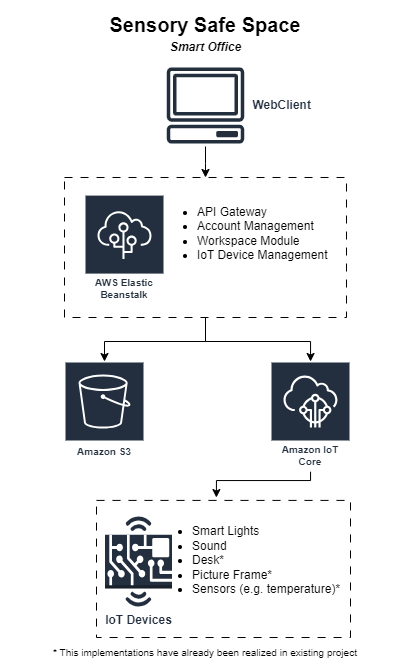
\includegraphics[height=3.5cm]{fig/SchmematicAwsV5-Seite-3.drawio.png}
		\caption{Architektur des Smart-Office-Prototyps}
		\label{fig:schematic-prototype}
\end{figure}

%%%%%%%%%%%%%%%%%%%%%%%%%%%%%%%%%%%%%%%%%%%%%%%%%%%%%%%%%%%%%%%%%%%%%%%%%%%%%%%%%%%%%%%%%%%%%%%
% TODO: Erster Entwurf der Kernkomponenten und Evaluierungsmethoden
%%%%%%%%%%%%%%%%%%%%%%%%%%%%%%%%%%%%%%%%%%%%%%%%%%%%%%%%%%%%%%%%%%%%%%%%%%%%%%%%%%%%%%%%%%%%%%%	

\subsubsection{Kernkomponenten}
*Die Kernkomponenten des Prototyps umfassen AWS-basierte Services, die die grundlegenden Funktionen des Systems bereitstellen.
AWS Elastic Beanstalk dient als Host für die Backend Logik und ....  Das API Gateway dient als Schnittestelle zwischen WebClient 
und IoT-Geräten und verwendet  z.B. Zigbee-API, MQTT, ... * und sorgt für eine reibungslose Kommunikation zwischen den Komponenten.
Die IoT Device Management Komponente sorgt für die Verwaltung der Geräte (z.B. Smart Lights, Desk, Picture Frame), sowie die 
zielgruppenspezifischen Erweiterungen (z.B. Lichtsteuerung, Akustik, Dashboard). Dabei dient Amazon S3 als Speicher für Nutzerdaten
(Opt-in) und Sensorwerte.


\subsubsection{Erweiterungen für Zielgruppen}
Diese Komponenten sind spezifisch für die zielgruppengerichtete Anpassung des Systems dienlich und werden über die 
Kernkomponenten hinaus implementiert. Philips Hue-Lampen (oder sonst iwelche Smart Lights) passen sich via Zigbee-API
an Tageszeit und Nutzerprofile an (z.B. warmes Licht für Autist:innen). Ein Raspberry Pi oder Microcontroller (oder sonstige Hardware)
mit Noise-Cancelling-Software generiert individuell angepasste Soundscapes (z.B. Weißes Rauschen für ADHS-Betroffene).
React-basierte Oberfläche mit drag-and-drop-Tagesplaner und Priorisierungsalgorithmus (Eisenhower-Matrix)....


\subsection{Evaluationsmethoden}

\subsubsection{DELTA Analyse}
Hier soll verglichen werden welche Veränderungen sich von \cite{ref01}{Towards a Cloud-Based Smart Office 
Solution for Shared Workplace Individualization} durch die zielgruppenspezifische Erweriterung ergeben


\subsubsection{Performance-Messung}
Um die Wirksamkeit des Systems zu validieren, werden folgende Metriken und Tools eingesetzt:
AWS CloudWatch überwacht Antwortzeiten der IoT-Geräte (Ziel: <500 ms für Echtzeit-Anpassungen).
Lasttests mit JMeter simulieren bis zu 1.000 gleichzeitige Nutzer:innen


\subsubsection{Usability und Accessibility}
\begin{itemize}
    \item \textbf{WCAG 2.1-Konformität}: Automatisierte Tests mit Axe und WAVE validieren Barrierefreiheit.
  
%%%%%%%%%%%%%%%%%%%%%%%%%%%%%%%%%%%%%%%%%%%%%%%%%%%%%%%%%%%%%%%%%%%%%%%%%%%%%%%%%%%%%%%%%%%%
%% Tools die sich anbieten würden hierfür:
%% https://sparkbox.com/foundry/lighthouse_chrome_website_accessibility_audit_website_accessibility_checker
%%	https://www.deque.com/axe/
%%%%%%%%%%%%%%%%%%%%%%%%%%%%%%%%%%%%%%%%%%%%%%%%%%%%%%%%%%%%%%%%%%%%%%%%%%%%%%%%%%%%%%%%%%%%

vllcht light/Dark mode -- Lichtempfindlichkeit Autist:innen
Generierung eines quantitativen Accessibility-Scores pro Komponente (z.B. 95/100 für das Dashboard) - 
Ein Accessibility-Score ist eine Zahl zwischen 0 und 100, die angibt, wie barrierefrei eine Komponente
 (z.B. ein Button, ein Formular oder das gesamte Dashboard) ist.
 Beispiel:
 95/100: Die Komponente erfüllt fast alle Kriterien, hat aber geringfügige Verbesserungspotenziale.
  70/100: Es gibt deutliche Mängel, die bestimmte Nutzer:innen ausschließen (z.B. fehlende Alt-Texte).

\end{itemize}

Der methodische Ansatz kombiniert technische Agilität (AWS, IoT) mit psychologischer Prävention und ethischer Verantwortung. 
Durch die Integration verschiedener Komponenten aus \cite{ref01}{Towards a Cloud-Based Smart Office Solution for Shared Workplace 
Individualization} und den zielgruppenspezifischen Erweiterungen wird eine intersektionale Plattform geschaffen, die Inklusion 
in der Arbeitswelt neu definieren könnte und die Bedürfnisse neurodivergenter Menschen und Burnout-Rückkehrer:innen berücksichtigt,
um diesen Gruppen ein angemessenes und inklusives Arbeitsumfeld zu schaffen.

\newpage
%Je nach dem in welcher Sprache ihr euer Paper schreiben wollt, benutzt bitte entweder den Deutschen-Titel oder den Englischen (einfach aus- bzw. einkommentieren mittels '%')

%Deutsch
\section{Schlussfolgerungen und Ausblick}


%Englisch
%\section{Conclusion and Future Work}

Mit dem letzten Kapitel schließt das Position Paper ab und sollte im Idealfall folgende Informationen beinhalten:
\begin{itemize}
	\item Erinnert den Leser / die Leserin in welchem Universum / Forschungsfeld das Position Paper ist
	\item Erinnert den Leser / die Leserin was die Problemstellung in diesem Universum / Forschungsfeld
	\item Erinnert den Leser / die Leserin an die vorgeschlagene Herangehensweise aus Kapitel 3, wie ihr vor habt diese Problemstellung zu bearbeiten
	\item gebt dem Leser / der Leserin die wichtigesten Key-Points eures Papers mit (bevor sie aufhören zu lesen), so dass sie sich "ewig" daran erinnern bzw. eure Ideen weitererzählen
	\item gebt dem Leser / der Leserin einen Ausblick (Future Work) was ihr als nächstes tun werdet (einen Vorgeschmack auf das Final Paper)
\end{itemize}

\vspace{10pt}
\textbf{VORGABE}: dieses Kapitel soll nicht mehr als eine A4-Seite benötigen

\vspace{10pt}
Hier noch ein paar Position Paper (Beispiel) and denen ihr euch orientieren könnt:
\begin{itemize}
	\item\textbf{\textit{Paper \cite{ref01}}:} \\
	Igor Ivki\'c, Andreas Mauthe, and Markus Tauber. (2019). 
	\textit{"Towards a Security Cost Model for Cyber-Physical Systems"}. In Proceedings of the 16th Annual Consumer Communications \& Networking Conference (CCNS). 
	IEEE.\\
	\textbf{Beschreibung:} soll als Vorlage dienen, wie ein Position Paper aufgebaut sein kann\\
	\textbf{Link:} \href{https://arxiv.org/pdf/1905.06124.pdf}{https://arxiv.org/pdf/1905.06124.pdf}\\
	\item\textbf{\textit{Paper \cite{ref02}}:} \\
	Igor Ivki\'c, Harald Pichler, Mario Zsilak, Andreas Mauthe, and Markus Tauber. (2019). 
	\textit{“A Framework for Measuring the Costs of Security at Runtime”}. 
	In Proceedings of the 9th International Conference on Cloud Computing and Services Science (CLOSER).\\
	\textbf{Beschreibung:} soll als Vorlage dienen, wie ein Position Paper aufgebaut sein kann. \\
	\textbf{Link:} \href{https://arxiv.org/pdf/1905.11180.pdf}{https://arxiv.org/pdf/1905.11180.pdf}\\
	
	\item\textbf{\textit{Paper \cite{ref03}}:} \\
	Igor Ivki\'c, Patrizia Sailer, Antonios Gouglidis, Andreas Mauthe, and Markus Tauber. (2021).
	\textit{"A Security Cost Modelling Framework for Cyber- Physical Systems"}.
	ACM Transactions on Internet Technology (TOIT).\\
	\textbf{Beschreibung:} soll als Vorlage dienen, wie man ein Related Work Kapitel aufziehen kann. Dieses Paper ist ein Journal-Artikel und untersucht ein Thema in der Tiefe. Im Vergleich dazu soll bei einem Position Paper ein neues Thema motiviert werden und der Anreiz geschaffen werden, dass es wichtig wäre, dies genauer zu untersuchen. \\
	\textbf{Link:} \href{https://arxiv.org/pdf/2107.07784.pdf}{https://arxiv.org/pdf/2107.07784.pdf}\\
\end{itemize}

\newpage
Hier ist noch ein Beispiel, wie man eine Grafik einfügt:
\begin{figure}[H]
	\centering
	
\includegraphics[width=10cm]{fig/Fig1.png}
	\caption{Master Cloud Computing Engineering (MCCE).}
	\Description{MCCE.}
	\label{fig:Fig1}
\end{figure}
\newpage
%% The next two lines define the bibliography style to be used, and
%% the bibliography file.
\bibliographystyle{apalike}
\bibliography{section/references}

\end{document}
\endinput
%%
%% End of file `sample-acmlarge.tex'.
